\documentclass{standalone}
\usepackage{tikz}
\usetikzlibrary{patterns, positioning}
\usepackage[sfdefault]{ClearSans} %% option 'sfdefault' activates Clear Sans as the default text font
\usepackage[T1]{fontenc}

\begin{document}
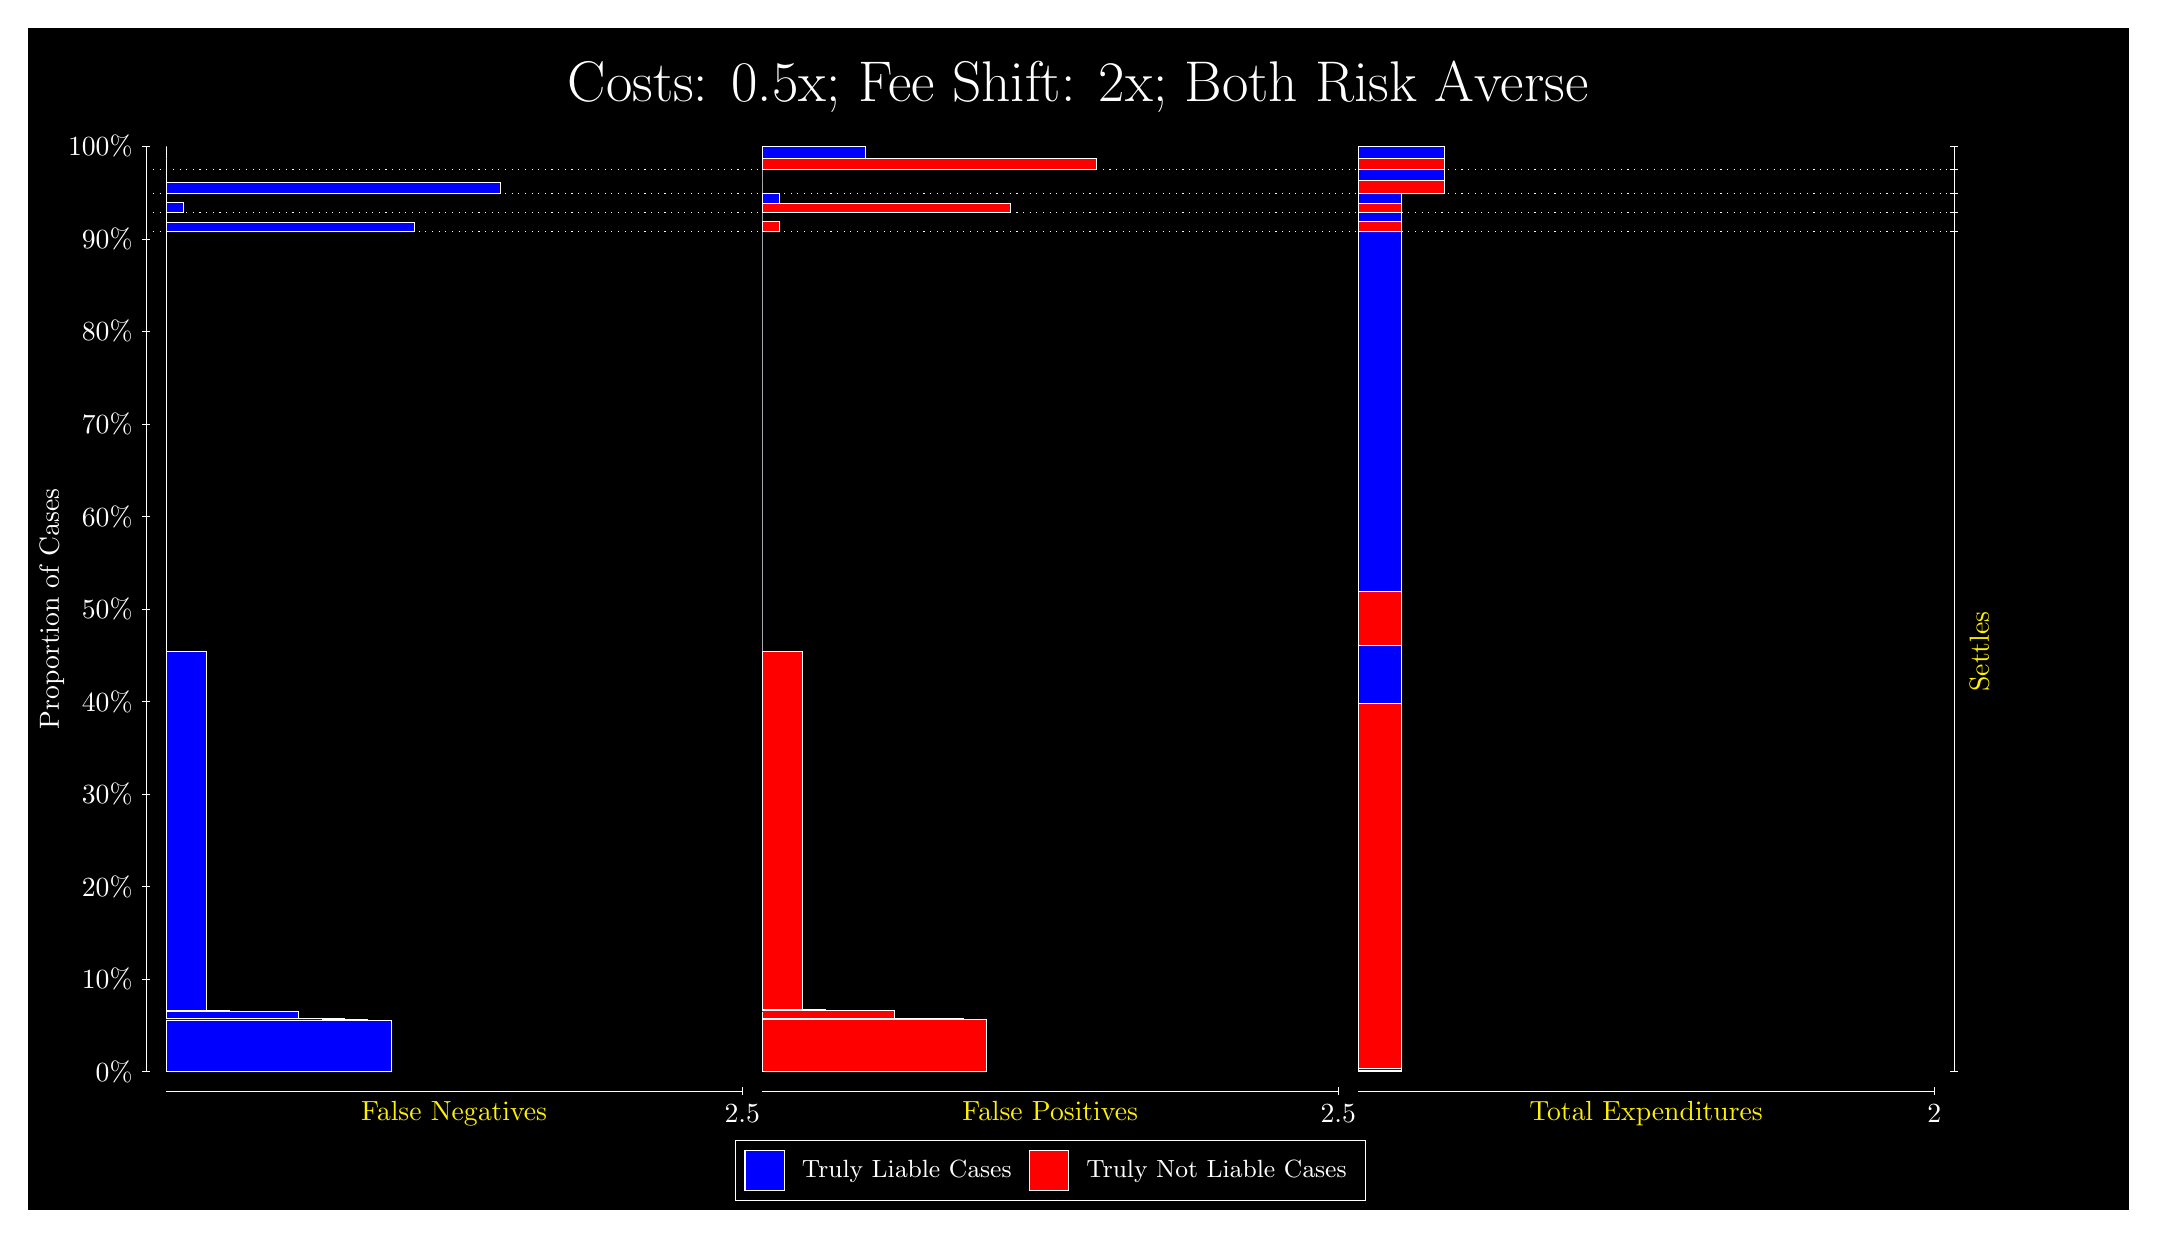
\begin{tikzpicture}
\draw[fill=black] (0,0) rectangle (26.667,15);
\draw[text=white] (0,13.5) rectangle (26.667,15) node[midway] {\huge Costs: 0.5x; Fee Shift: 2x; Both Risk Averse};
\draw[white, very thin] (1.5,1.75) -- (1.5,13.5);
\node[rotate=90, text=white, anchor=center] at (0.3, 7.625) {Proportion of Cases};
\draw[white, very thin] (1.45,1.75) -- (1.55,1.75);
\node[text=white, anchor=east] at (1.45, 1.75) {0\%};
\draw[white, very thin] (1.45,2.925) -- (1.55,2.925);
\node[text=white, anchor=east] at (1.45, 2.925) {10\%};
\draw[white, very thin] (1.45,4.1) -- (1.55,4.1);
\node[text=white, anchor=east] at (1.45, 4.1) {20\%};
\draw[white, very thin] (1.45,5.275) -- (1.55,5.275);
\node[text=white, anchor=east] at (1.45, 5.275) {30\%};
\draw[white, very thin] (1.45,6.45) -- (1.55,6.45);
\node[text=white, anchor=east] at (1.45, 6.45) {40\%};
\draw[white, very thin] (1.45,7.625) -- (1.55,7.625);
\node[text=white, anchor=east] at (1.45, 7.625) {50\%};
\draw[white, very thin] (1.45,8.8) -- (1.55,8.8);
\node[text=white, anchor=east] at (1.45, 8.8) {60\%};
\draw[white, very thin] (1.45,9.975) -- (1.55,9.975);
\node[text=white, anchor=east] at (1.45, 9.975) {70\%};
\draw[white, very thin] (1.45,11.15) -- (1.55,11.15);
\node[text=white, anchor=east] at (1.45, 11.15) {80\%};
\draw[white, very thin] (1.45,12.325) -- (1.55,12.325);
\node[text=white, anchor=east] at (1.45, 12.325) {90\%};
\draw[white, very thin] (1.45,13.5) -- (1.55,13.5);
\node[text=white, anchor=east] at (1.45, 13.5) {100\%};

\draw[white, very thin] (24.457,1.75) -- (24.457,13.5);
\draw[white, very thin] (24.407,1.75) -- (24.507,1.75);
\node[anchor=west] at (24.407, 1.75) {};
\draw[white, very thin] (24.407,12.418) -- (24.507,12.418);
\node[anchor=west] at (24.407, 12.418) {};
\draw[white, very thin] (24.407,12.662) -- (24.507,12.662);
\node[anchor=west] at (24.407, 12.662) {};
\draw[white, very thin] (24.407,12.906) -- (24.507,12.906);
\node[anchor=west] at (24.407, 12.906) {};
\draw[white, very thin] (24.407,13.203) -- (24.507,13.203);
\node[anchor=west] at (24.407, 13.203) {};
\draw[white, very thin] (24.407,13.5) -- (24.507,13.5);
\node[anchor=west] at (24.407, 13.5) {};

\draw[white, very thin, fill=blue] (1.75,1.75) rectangle (4.6044,2.4036);
\draw[white, very thin, fill=blue] (1.75,2.4036) rectangle (4.3116,2.4167);
\draw[white, very thin, fill=blue] (1.75,2.4167) rectangle (4.0188,2.4213);
\draw[white, very thin, fill=blue] (1.75,2.4213) rectangle (3.7261,2.4227);
\draw[white, very thin, fill=blue] (1.75,2.4227) rectangle (3.4333,2.5153);
\draw[white, very thin, fill=blue] (1.75,2.5153) rectangle (3.1406,2.5183);
\draw[white, very thin, fill=blue] (1.75,2.5183) rectangle (2.8478,2.5213);
\draw[white, very thin, fill=blue] (1.75,2.5213) rectangle (2.5551,2.5307);
\draw[white, very thin, fill=blue] (1.75,2.5307) rectangle (2.2623,7.084);
\draw[white, very thin, fill=red] (1.75,7.084) rectangle (1.75,12.418);
\draw[white, very thin, fill=blue] (1.75,12.418) rectangle (4.8971,12.536);
\draw[white, very thin, fill=red] (1.75,12.536) rectangle (1.75,12.662);
\draw[white, very thin, fill=blue] (1.75,12.662) rectangle (1.9696,12.787);
\draw[white, very thin, fill=red] (1.75,12.787) rectangle (1.75,12.906);
\draw[white, very thin, fill=blue] (1.75,12.906) rectangle (5.9949,13.046);
\draw[white, very thin, fill=red] (1.75,13.046) rectangle (1.75,13.203);
\draw[white, very thin, fill=red] (1.75,13.203) rectangle (1.75,13.343);
\draw[white, very thin, fill=blue] (1.75,13.343) rectangle (1.75,13.5);
\draw[white, very thin, fill=red] (9.3189,1.75) rectangle (12.173,2.4164);
\draw[white, very thin, fill=red] (9.3189,2.4164) rectangle (11.88,2.4247);
\draw[white, very thin, fill=red] (9.3189,2.4247) rectangle (11.588,2.4275);
\draw[white, very thin, fill=red] (9.3189,2.4275) rectangle (11.295,2.4302);
\draw[white, very thin, fill=red] (9.3189,2.4302) rectangle (11.002,2.523);
\draw[white, very thin, fill=red] (9.3189,2.523) rectangle (10.709,2.5233);
\draw[white, very thin, fill=red] (9.3189,2.5233) rectangle (10.709,2.5246);
\draw[white, very thin, fill=red] (9.3189,2.5246) rectangle (10.417,2.5297);
\draw[white, very thin, fill=red] (9.3189,2.5297) rectangle (10.124,2.5444);
\draw[white, very thin, fill=red] (9.3189,2.5444) rectangle (9.8312,7.0838);
\draw[white, very thin, fill=blue] (9.3189,7.0838) rectangle (9.3189,12.418);
\draw[white, very thin, fill=red] (9.3189,12.418) rectangle (9.5384,12.543);
\draw[white, very thin, fill=blue] (9.3189,12.543) rectangle (9.3189,12.662);
\draw[white, very thin, fill=red] (9.3189,12.662) rectangle (12.466,12.781);
\draw[white, very thin, fill=blue] (9.3189,12.781) rectangle (9.5384,12.906);
\draw[white, very thin, fill=red] (9.3189,12.906) rectangle (9.3189,13.063);
\draw[white, very thin, fill=blue] (9.3189,13.063) rectangle (9.3189,13.203);
\draw[white, very thin, fill=red] (9.3189,13.203) rectangle (13.564,13.343);
\draw[white, very thin, fill=blue] (9.3189,13.343) rectangle (10.636,13.5);
\draw[white, very thin, fill=red] (16.888,1.75) rectangle (17.437,1.7713);
\draw[white, very thin, fill=blue] (16.888,1.7713) rectangle (17.437,1.7905);
\draw[white, very thin, fill=red] (16.888,1.7905) rectangle (17.437,6.4227);
\draw[white, very thin, fill=blue] (16.888,6.4227) rectangle (17.437,7.1689);
\draw[white, very thin, fill=red] (16.888,7.1689) rectangle (17.437,7.8491);
\draw[white, very thin, fill=blue] (16.888,7.8491) rectangle (17.437,12.418);
\draw[white, very thin, fill=red] (16.888,12.418) rectangle (17.437,12.543);
\draw[white, very thin, fill=blue] (16.888,12.543) rectangle (17.437,12.662);
\draw[white, very thin, fill=red] (16.888,12.662) rectangle (17.437,12.781);
\draw[white, very thin, fill=blue] (16.888,12.781) rectangle (17.437,12.906);
\draw[white, very thin, fill=red] (16.888,12.906) rectangle (17.986,13.063);
\draw[white, very thin, fill=blue] (16.888,13.063) rectangle (17.986,13.203);
\draw[white, very thin, fill=red] (16.888,13.203) rectangle (17.986,13.343);
\draw[white, very thin, fill=blue] (16.888,13.343) rectangle (17.986,13.5);
\draw[white, dotted] (1.5,12.418) -- (24.457,12.418);
\draw[white, dotted] (1.5,12.662) -- (24.457,12.662);
\draw[white, dotted] (1.5,12.906) -- (24.457,12.906);
\draw[white, dotted] (1.5,13.203) -- (24.457,13.203);
\draw[white, very thin] (1.75,1.5) -- (9.0689,1.5);
\node[text=yellow, anchor=north] at (5.4094, 1.5) {False Negatives};
\draw[white, very thin] (9.0689,1.45) -- (9.0689,1.55);
\node[text=white, anchor=north] at (9.0689, 1.45) {2.5};

\draw[white, very thin] (9.3189,1.5) -- (16.638,1.5);
\node[text=yellow, anchor=north] at (12.978, 1.5) {False Positives};
\draw[white, very thin] (16.638,1.45) -- (16.638,1.55);
\node[text=white, anchor=north] at (16.638, 1.45) {2.5};

\draw[white, very thin] (16.888,1.5) -- (24.207,1.5);
\node[text=yellow, anchor=north] at (20.547, 1.5) {Total Expenditures};
\draw[white, very thin] (24.207,1.45) -- (24.207,1.55);
\node[text=white, anchor=north] at (24.207, 1.45) {2};

\node[text=yellow, centered, rotate=90] at (24.777, 7.0839) {Settles};





\draw (12.978300999999998,1.5) node[draw=none] (baseCoordinate) {};
\begin{scope}[align=center]
        \matrix[scale=0.5, draw=white, below=0.5cm of baseCoordinate, nodes={draw}, column sep=0.1cm]{
            \node[rectangle, draw, minimum width=0.5cm, minimum height=0.5cm, fill=blue] {}; &
            \node[draw=none, font=\small, text=white] (B) {Truly Liable Cases}; &
            \node[rectangle, draw, minimum width=0.5cm, minimum height=0.5cm, fill=red] {}; &
            \node[draw=none, font=\small, text=white] (B) {Truly Not Liable Cases}; \\
            };
\end{scope}

\end{tikzpicture}
\end{document}